%=============================================================================
\section{Design}

%-----------------------------------------------------------------------------
\subsection{Approach}

\enote{Explain data flow; calling approach based on passing buffers; in-process or cross-process. Explain using FlatBuffers and why. Explain in general terms that we deal directly with variables in a global space, with lightweight coordination to allocate variables; and why (avoid duplication/rewriting etc.}

zkInterface is a procedural, purely functional interface for zero-knowledge systems that enables cross-language interoperability via dynamic linking and shared memory. The current version, even if limiting, creates an interface based on R1CS formatting and offers the ability to abstractly craft a constraint system building from different components, possibly written in different frameworks, by determining how data should be written and read. 

\enote{I'm not sure what this means:}
It can also be seen as a design tool for improved generation of constraints and usability, analogous to a portable binary format, since one can parametrize the functions calls and easily compose different functions, or components, that are not directly compatible.

\begin{figure}[h!]
	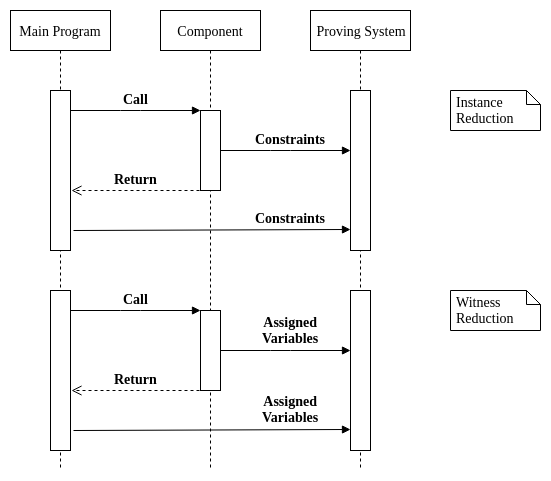
\includegraphics[width=\linewidth]{call_flow.png}
	\caption{The flow of messages between libraries using the interface}
	\label{flow}
\end{figure}


\subsection{Architecture}

\enote{Describe the high-level design, introducing all the main concepts in a readable narrative and referring to them concretely by the  identifier name in the sourcecode.}

\paragraph{Interface.}

	The interface is defined as a set of messages that the caller and callee can exchange.
	The definition is provided in Listing \ref{gadget.fbs} as a FlatBuffers schema.
	Refer to the inline documentation of each message and field.

	\subparagraph{Note}
	The FlatBuffers system includes a simple interface definition language,
	a data layout specification,
	a clear evolution path for future extensions of the standard,
	support for all common programming languages,
	and the possibility of very efficient implementations.
	The specification of FlatBuffers can be found at
	\href{https://google.github.io/flatbuffers/}{https://google.github.io/flatbuffers/}.

\paragraph{Messages Flow.}

	The flow of messages is illustrated in Figure \ref{flow}.

	The caller calls the component code with a single Call message.
	The component exits with a single Return message.
	This is a control flow analoguous to a function call in common programming languages.

	The caller also provides a way for the component to send 
	R1CSConstraints and AssignedVariables messages.
	This is an output channel distinct from the return message.

	During instance reduction,
	a component may add any number of constraints to the constraint system
	by sending one or more R1CSConstraints messages.
	The caller and other components may do so as well.

	During witness reduction,
	a component may assign values to variables
	by sending one or more AssignedVariables messages.

	\subparagraph{Note}
	The design of constraints and assignments channels
	allows a component to call subcomponents itself.
	Messages from all (sub-)components can simply be sent separately
	without the need to aggregate them into a single message.
	
	Moreover, an implementation can decouple the proving system
	from the logic of building constraints and assignments,
	by arranging for the constraints and assignments messages
	to be processed by the proving system, independently from the control logic.

\paragraph{Variables.}

	All variables in a constraint system are assigned a numerical identifier
	unique within this system.
	Messages that contain constraints or assignments refer to variables by their
	unique ID.

	\subparagraph{Note}
	This design allows implementations to aggregate and handle messages in a generic way,
	without any	reference to the components or mechanisms that generated them.

	\anote{Must be consecutive or are gaps allowed?}

\paragraph{Local Variables Allocation.}

	A component may allocate a number of local variables to use
	in the internal implementation of the function that it computes.
	They are analoguous to stack variables in common programming languages.

	The following protocol is used to allocate variable IDs that are
	unique within a whole constraint system.
	\begin{itemize}
		\item The caller must provide a numerical ID greater than all IDs that have already been allocated, called the Free-Before ID.
		\item The component may use the Free-Before ID and consecutive IDs as its local variables IDs.
		\item The component must return the next consecutive ID that it did not use, called the Free-After ID.
		\item The caller must treat IDs lesser than the Free-After ID as allocated by the component,
			and must not use them.
	\end{itemize}

	During instance reduction, the component can refer to
	its local variables in the R1CSConstraints messages that it generates.
	The caller and other parts of the program must not refer to these local variables.

	During witness reduction, the component must assign values to its local variables
	by sending AssignedVariables messages.

\paragraph{Incoming/Outgoing Variables.}

	The concept of incoming, outgoing variables arises when a program is decomposed into components.
	These variables serve as the functional interface between a component and its caller.
	They are analoguous to arguments and return values of functions in common programming languages.
	A variable is not inherently incoming, outgoing, nor local;
	rather, this is a convention in the context of a component call.

	The caller provides the IDs of variables to be used as incoming and outgoing variables by the component.
	There may be no outgoing variables if the component implements a pure assertion.

	During instance reduction, both the caller and the component can refer to
	these variables in the R1CSConstraints messages that they generate.
	Other parts of the program may also refer to these same variables in their own contexts.

	During witness reduction, the caller must pass incoming values to the component in the Call message.
	The component must return outgoing values to the caller in the Return message.

	The caller is responsible for the assignment of values to both incoming and outgoing variables.
	How this is achieved depends on the caller and proving system,
	and on whether some variables are treated as public inputs of the zero-knowledge program.

\paragraph{C Interface.}

	A C interface to exchange messages is defined in Listing \ref{gadget.h}.
	Refer to the inline documentation.

\paragraph{Stream and File Format.}
	\enote{Explain what's already induced by FlatBuffers: explain that the framework, plus our .fbs file, specify how the aforementioned high-level messages are actually represented at the byte level, including message framing, message naming, etc..}
	All messages are framed, meaning that they can be concatenated and distinguished in streams of bytes or in files.
	Messages must be prefixed by the size of the message not including the prefix,
	as a 4-bytes little-endian unsigned integer.
	\enote{Say something about streams - stdio/stdout, files, TCP connections, etc.?}
